% !TEX root = ../main.tex
\documentclass[../main.tex]{subfiles}

\begin{document}
\section{Z-Diode für Spannungsstabilisierung erweitert mit BJT}

\subsection{Ziel}

Als eine Erweiterung zur Zenerdiodenstabilisierung aus Labor 1, wird in dieser Schaltung ein Transistor \textit{BC548B} als Längsregler verwendet. Es soll gezeigt werden, wie sich die Line- \& Load-Regulation im Vergleich zur Schaltung ohne Transistor verhält.

\subsection{Berechnungen}
Die Vorgaben für die Schaltung sind eine variable Eingangsspannung $\SI{10}{\volt} \le U_s \le \SI{16}{\volt}$ und eine Variable Last $\SI{0}{\milli\ampere} \le I_{Last} \le \SI{10}{\milli\ampere}$.

Der Transistor wird in dieser Schaltung gesättigt betrieben. Mit dem über Gleichung \ref{equ:zbjt_Ib} berechneten Basistrom, in Summe mit dem minimalen Z-Dioden-Strom $I_Z = \SI{5}{\milli\ampere}$, und der minimalen Speisspannung $U_{s_{min}} = 10V$ errechnet sich über Gleichung \ref{equ:zbjt_Rv} ein Vorwiderstand von $R_v = \SI{820}{\ohm}$.

\begin{equation}
    I_{B} = \frac{I_C}{h_{FE_{min}}} \cdot {"u} = \frac{\SI{10}{\milli\ampere}}{200} \cdot 3=\SI{150}{\micro\ampere}
    \label{equ:zbjt_Ib}
\end{equation}

\begin{equation}
    R_{V} = \frac{U_{s_{min}} - U_Z}{I_B + I_Z} = \frac{\SI{10}{\volt} - \SI{5.6}{\volt}}{\SI{150}{\micro\ampere} + \SI{5}{\milli\ampere}} = \SI{854}{\ohm} \Rightarrow \textrm{E12-Reihe } R_{V} = \SI{820}{\ohm}
    \label{equ:zbjt_Rv}
\end{equation}

Die Lastspannung beträgt $\approx\SI{5}{\volt}$ bei einer Basisemitter-Spannung von $U_{BE} \approx \SI{0.6}{V}$. Messungen werden mit den drei Lastströmen $I_L = \SI{0}{\milli\ampere}, \SI{5}{\milli\ampere}, \SI{10}{\milli\ampere}$ durchgeführt. Dafür werden nach $U=R \cdot I$ die zwei Lastwiderstände $R_L = \SI{1}{\kilo\ohm}, \SI{470}{\ohm}$ \& einmal lastlos verwendet.

\subsection{Messschaltung}

\begin{figure}[h]
    \centering
    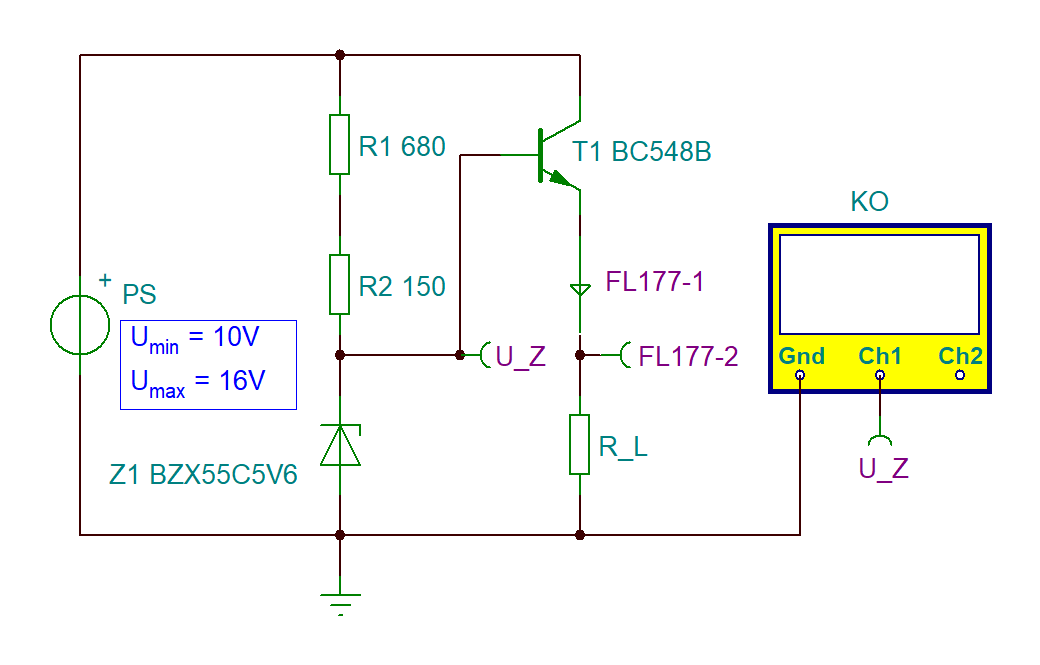
\includegraphics[scale=0.35]{assets/task2_voltage_stable/messschaltung_task2.PNG}
    \caption{Spannungsstabilisierung mit Z-Diode \& BJT}
    \label{fig:circuit_voltage_stabilization}
\end{figure}

\subsection{Resultate Line Regulation}


\begin{table}[h]
\renewcommand{\arraystretch}{1.3}
\centering
\begin{tabular}{l|llll}
\textbf{$U_S$} $[\si{\volt}]$ & \textbf{$U_Z$} $[\si{\volt}]$ & \textbf{$I_V$} $[\si{\milli\ampere}]$ & \textbf{$U_L$} $[\si{\volt}]$ & \textbf{$I_L (R_L = \SI{470}{\ohm})$} $[\si{\milli\ampere}]$\\ \hline
10.00       & 5.68        & 1.63        & 4.89        & 10.37       \\
11.00       & 5.71        & 2.54        & 4.95        & 10.46       \\
12.00       & 5.71        & 4.54        & 4.94        & 10.46       \\
13.00       & 5.71        & 5.49        & 4.95        & 10.51       \\
14.00       & 5.74        & 6.46        & 4.97        & 10.54       \\
15.00       & 5.74        & 7.42        & 4.99        & 10.58       \\
16.00       & 5.74        & 9.44        & 4.99        & 10.56      

\end{tabular}
\caption{Messresultate mit $\SI{470}{\ohm}$ Lastwiderstand}
\label{tab:result_task2_R680}
\end{table}

\begin{equation}
    \text{line regulation} = \frac{\Delta U_{L}}{\Delta U_{S}} = \frac{\SI{4.99}{\volt}-\SI{4.89}{\volt}}{\SI{16}{\volt} - \SI{10}{\volt}} = \frac{1}{60} = 0.016\bar{6}\ (\text{TINA} \Rightarrow 0.018)
    \label{equ:task2_line_reg_680R}
\end{equation}

\begin{table}[h]
\renewcommand{\arraystretch}{1.3}
\centering
\begin{tabular}{l|llll}
\textbf{$U_S$} $[\si{\volt}]$ & \textbf{$U_Z$} $[\si{\volt}]$ & \textbf{$I_V$} $[\si{\milli\ampere}]$ & \textbf{$U_L$} $[\si{\volt}]$ & \textbf{$I_L (R_L = \SI{1}{\kilo\ohm})$} $[\si{\milli\ampere}]$\\  \hline
10.00       & 5.68        & 2.03        & 4.92        & 4.97 \\
11.00       & 5.68        & 3.02        & 4.93        & 4.98 \\
12.00       & 5.68        & 5.01        & 4.94        & 4.99 \\
13.00       & 5.71        & 6.00        & 4.95        & 5.00 \\
14.00       & 5.71        & 5.99        & 4.96        & 5.01 \\
15.00       & 5.71        & 7.98        & 4.97        & 5.02 \\
16.00       & 5.71        & 8.97        & 4.98        & 5.03 
\end{tabular}
\caption{Messresultate mit $\SI{1}{\kilo\ohm}$ Lastwiderstand}
\label{tab:result_task2_R1k}
\end{table}

\begin{equation}
    \text{line regulation} = \frac{\Delta U_{L}}{\Delta U_{S}} = \frac{\SI{4.98}{\volt}-\SI{4.92}{\volt}}{\SI{16}{\volt} - \SI{10}{\volt}} = 0.01 \ (\text{TINA} \Rightarrow 0.018)
    \label{equ:task2_line_reg_1k}
\end{equation}

\newpage

\begin{table}[h]
\renewcommand{\arraystretch}{1.3}
\centering
\begin{tabular}{l|llll}
\textbf{$U_S$} $[\si{\volt}]$ & \textbf{$U_Z$} $[\si{\volt}]$ & \textbf{$I_V$} $[\si{\milli\ampere}]$ & \textbf{$U_L$} $[\si{\volt}]$ & \textbf{$I_L (R_L = \infty\ \si{\ohm})$} $[\si{\milli\ampere}]$\\  \hline
10.00       & 5.68      & 2.00        & 5.17        & 0.00                               \\
11.00       & 5.70      & 3.00        & 5.17        & 0.00                               \\
12.00       & 5.68      & 4.00        & 5.18        & 0.00                               \\
13.00       & 5.68      & 5.00        & 5.18        & 0.00                               \\
14.00       & 5.68      & 6.00        & 5.19        & 0.00                               \\
15.00       & 5.71      & 9.00        & 5.19        & 0.00                               \\
16.00       & 5.74      & 9.00        & 5.20        & 0.00                              
\end{tabular}
\caption{Messresultate ohne Lastwiderstand}
\label{tab:result_task2_line_reg_no_load}
\end{table}

\begin{equation}
    \text{line regulation} = \frac{\Delta U_{L}}{\Delta U_{S}} = \frac{\SI{5.20}{\volt}-\SI{5.17}{\volt}}{\SI{16}{\volt} - \SI{10}{\volt}} = 0.005 \ (\text{TINA} \Rightarrow 1.007)
    \label{equ:task2_line_reg_infty}
\end{equation}

\subsection{Resultate Load Regulation}

\begin{table}[h]
\renewcommand{\arraystretch}{1.3}
\centering
\begin{tabular}{l|ll}
\textbf{$R_L$} $[\si{\ohm}]$ & \textbf{$U_L$} $[\si{\volt}]$ & \textbf{$I_L$} $[\si{\milli\ampere}]$ \\ \hline
\textbf{$\SI{1}{\kilo\ohm}$}    & 4.92  & 4.97    \\
\textbf{$\SI{680}{\ohm}$}       & 4.89  & 10.4  
\end{tabular}
\caption{Messresultate $U_S = \SI{10}{\volt}$}
\label{tab:result_task2_load_reg_10V}
\end{table}

\begin{equation}
    \text{load regulation} = \frac{\Delta U_{L}}{\Delta I_{L}} = \frac{\SI{4.89}{\volt}-\SI{4.92}{\volt}}{\SI{10.4}{\milli\ampere} - \SI{4.97}{\milli\ampere}} = -6.3 \frac{\si{\volt}}{\si{\ampere}}
    \label{equ:task2_load_reg_10V}
\end{equation}

\begin{table}[h]
\renewcommand{\arraystretch}{1.3}
\centering
\begin{tabular}{l|ll}
\textbf{$R_L$} $[\si{\ohm}]$ & \textbf{$U_L$} $[\si{\volt}]$ & \textbf{$I_L$} $[\si{\milli\ampere}]$ \\ \hline
\textbf{$\SI{1}{\kilo\ohm}$}    & 4.98  & 5.03    \\
\textbf{$\SI{680}{\ohm}$}       & 4.99  & 10.56  
\end{tabular}
\caption{Messresultate $U_S = \SI{16}{\volt}$}
\label{tab:result_task2_load_reg_16V}
\end{table}

\begin{equation}
    \text{load regulation} = \frac{\Delta U_{L}}{\Delta I_{L}} = \frac{\SI{4.99}{\volt}-\SI{4.99}{\volt}}{\SI{10.56}{\milli\ampere} - \SI{5.03}{\milli\ampere}} = 1.8 \frac{\si{\volt}}{\si{\ampere}}
    \label{equ:task2_load_reg_16V}
\end{equation}

\subsection{Schlussfolgerung}

Wird die \textit{Line Regulation} der Messungen mit den TINA-Werten verglichen, ist der Wert bei der kleineren Last (\SI{680}{\ohm}) näher an der Simulation, als bei der grösseren Last (\SI{1}{\kilo\ohm}). Bei Lastlos, ist die \textit{Line Regulation} stark daneben. Dies hat wohl den Grund, dass die Simulation die lastlose Spannung anders betrachtet als in der Realität. Anstatt die Limitierung durch die Z-Diode und die Abfallspannung über die Basis-Emitter-Pins, werden in der Simulation $U_{CE} \approx \SI{0.2}{\volt}$ von der Speisspannung abgezogen. Warum genau TINA dies macht, ist unserseits unbekannt.

Bei der \textit{Load Regulation} sehen wir, dass sich diese bei steigender Speisspannung verbessert. Optimal wären $\SI{0}{\frac{\si{\volt}}{\si{\ampere}}}$..
\end{document}